%%%%%%%%%%%%%%%%%%%%%%%%%%%%%%%%%%%%%%%%%
% Proceedings of the National Academy of Sciences (PNAS)
% LaTeX Template
% Version 1.0 (19/5/13)
%
% This template has been downloaded from:
% http://www.LaTeXTemplates.com
%
% Original author:
% The PNAStwo class was created and is owned by PNAS:
% http://www.pnas.org/site/authors/LaTex.xhtml
% This template has been modified from the blank PNAS template to include
% examples of how to insert content and drastically change commenting. The
% structural integrity is maintained as in the original blank template.
%
% Original header:
%% PNAStmpl.tex
%% Template file to use for PNAS articles prepared in LaTeX
%% Version: Apr 14, 2008
%
%%%%%%%%%%%%%%%%%%%%%%%%%%%%%%%%%%%%%%%%%
%----------------------------------------------------------------------------------------
%	PACKAGES AND OTHER DOCUMENT CONFIGURATIONS
%----------------------------------------------------------------------------------------

%------------------------------------------------
% BASIC CLASS FILE
%------------------------------------------------

%% PNAStwo for two column articles is called by default.
%% Uncomment PNASone for single column articles. One column class
%% and style files are available upon request from pnas@nas.edu.

%\documentclass{pnasone}
\documentclass{pnastwo}

%------------------------------------------------
% POSITION OF TEXT
%------------------------------------------------

%% Changing position of text on physical page:
%% Since not all printers position
%% the printed page in the same place on the physical page,
%% you can change the position yourself here, if you need to:

% \advance\voffset -.5in % Minus dimension will raise the printed page on the 
                         %  physical page; positive dimension will lower it.

%% You may set the dimension to the size that you need.

%------------------------------------------------
% GRAPHICS STYLE FILE
%------------------------------------------------

%% Requires graphics style file (graphicx.sty), used for inserting
%% .eps/image files into LaTeX articles.
%% Note that inclusion of .eps files is for your reference only;
%% when submitting to PNAS please submit figures separately.

%% Type into the square brackets the name of the driver program 
%% that you are using. If you don't know, try dvips, which is the
%% most common PC driver, or textures for the Mac. These are the options:

% [dvips], [xdvi], [dvipdf], [dvipdfm], [dvipdfmx], [pdftex], [dvipsone],
% [dviwindo], [emtex], [dviwin], [pctexps], [pctexwin], [pctexhp], [pctex32],
% [truetex], [tcidvi], [vtex], [oztex], [textures], [xetex]


%------------------------------------------------
% OPTIONAL POSTSCRIPT FONT FILES
%------------------------------------------------

%% PostScript font files: You may need to edit the PNASoneF.sty
%% or PNAStwoF.sty file to make the font names match those on your system. 
%% Alternatively, you can leave the font style file commands commented out
%% and typeset your article using the default Computer Modern 
%% fonts (recommended). If accepted, your article will be typeset
%% at PNAS using PostScript fonts.

% Choose PNASoneF for one column; PNAStwoF for two column:
%\usepackage{PNASoneF}
%\usepackage{PNAStwoF}

%------------------------------------------------
% ADDITIONAL OPTIONAL STYLE FILES
%------------------------------------------------

%% The AMS math files are commonly used to gain access to useful features
%% like extended math fonts and math commands.
\usepackage{multirow}
%\usepackage{caption}
%\usepackage{subcaption}
%\usepackage{etex}
\usepackage{color}
%\usepackage[usenames,dvipsnames,svgnames,table]{xcolor}
\usepackage[usenames,dvipsnames]{xcolor}
\usepackage{tikz}
\usetikzlibrary{decorations.shapes}
\usepackage{amssymb,amsfonts,amsmath}
\usepackage{xspace}
\newcommand{\dictionary}{\ensuremath{\mathcal{D}}\xspace}


%------------------------------------------------
% OPTIONAL MACRO FILES
%------------------------------------------------

%% Insert self-defined macros here.
%% \newcommand definitions are recommended; \def definitions are supported

%\newcommand{\mfrac}[2]{\frac{\displaystyle #1}{\displaystyle #2}}
%\def\s{\sigma}

%------------------------------------------------
% DO NOT EDIT THIS SECTION
%------------------------------------------------

%% For PNAS Only:
\contributor{Submitted to Proceedings of the National Academy of Sciences of the United States of America}
\url{www.pnas.org/cgi/doi/10.1073/pnas.0709640104}
\copyrightyear{2008}
\issuedate{Issue Date}
\volume{Volume}
\issuenumber{Issue Number}

%----------------------------------------------------------------------------------------

\begin{document}

%----------------------------------------------------------------------------------------
%	TITLE AND AUTHORS
%----------------------------------------------------------------------------------------

\title{Hyperbolically speaking: a computational model of non-literal language understanding} % For titles, only capitalize the first letter

%------------------------------------------------

%% Enter authors via the \author command.  
%% Use \affil to define affiliations.
%% (Leave no spaces between author name and \affil command)

%% Note that the \thanks{} command has been disabled in favor of
%% a generic, reserved space for PNAS publication footnotes.

%% \author{<author name>
%% \affil{<number>}{<Institution>}} One number for each institution.
%% The same number should be used for authors that
%% are affiliated with the same institution, after the first time
%% only the number is needed, ie, \affil{number}{text}, \affil{number}{}
%% Then, before last author ...
%% \and
%% \author{<author name>
%% \affil{<number>}{}}

%% For example, assuming Garcia and Sonnery are both affiliated with
%% Universidad de Murcia:
%% \author{Roberta Graff\affil{1}{University of Cambridge, Cambridge,
%% United Kingdom},
%% Javier de Ruiz Garcia\affil{2}{Universidad de Murcia, Bioquimica y Biologia
%% Molecular, Murcia, Spain}, \and Franklin Sonnery\affil{2}{}}

\author{Justine T. Kao\affil{1}{Stanford University},
Jean Wu,\affil{1}{}
Leon Bergen\affil{2}{MIT}
\and
Noah D. Goodman\affil{1}{}}

\contributor{Submitted to Proceedings of the National Academy of Sciences
of the United States of America}

%----------------------------------------------------------------------------------------

\maketitle % The \maketitle command is necessary to build the title page

\begin{article}

%----------------------------------------------------------------------------------------
%	ABSTRACT, KEYWORDS AND ABBREVIATIONS
%----------------------------------------------------------------------------------------

\begin{abstract}
One of the most intriguing and challenging properties of language understanding is that language is not always meant to be interpreted literally. In everyday situations, people often use imprecise, exaggerated, or otherwise literally false descriptions to communicate their experiences and opinions. In this paper we focus on the non-literal interpretation of number words, in particular the effects of
pragmatic halo (the imprecise interpretation of round numbers) and hyperbole (the affective subtext conveyed by exaggerated and unlikely numbers). Building on recent models of pragmatics as rational inference between speaker and listener, we model number interpretation as social inference regarding the communicative goal, meaning, and affective subtext of an utterance. Our model accurately predicts humans' pragmatic interpretation of number words, and is one of the first computational models to quantitatively capture a range of effects in non-literal language understanding.
\end{abstract}

%------------------------------------------------

\keywords{Pragmatics | Language understanding | Computational modeling} % When adding keywords, separate each term with a straight line: |

%------------------------------------------------

%% Optional for entering abbreviations, separate the abbreviation from
%% its definition with a comma, separate each pair with a semicolon:
%% for example:
%% \abbreviations{SAM, self-assembled monolayer; OTS,
%% octadecyltrichlorosilane}

% \abbreviations{}
%\abbreviations{IR, Incongruity Resolution}

%----------------------------------------------------------------------------------------
%	PUBLICATION CONTENT
%----------------------------------------------------------------------------------------

%% The first letter of the article should be drop cap: \dropcap{} e.g.,
%\dropcap{I}n this article we study the evolution of ''almost-sharp'' fronts

\section{Introduction}

\dropcap{I}magine a conversation with a friend about a new restaurant where she recently dined. Your friend says, ``It took $30$ minutes to get a table." You are likely to interpret this to mean she waited approximately $30$ minutes. Now suppose your friend says: ``It took $32$ minutes to get a table." You are more likely to interpret the number expression to mean exactly $32$, and believe that she cares to communicate the exact wait time. Suppose she says: ``It took a million hours to get a table." You will probably interpret her to mean that the wait was shorter than a million hours, but importantly that she thinks it took much too long. 

Given the incredible flexibility of language, a crucial part of a listener's job is to understand an utterance even when its literally meaning is extremely unlikely. Non-literal language understanding is one of the biggest challenges in language research, and it has been difficult to build formal models or design empirical studies that capture effects in non-literal language understanding quantitatively. In this paper, we present a computational model that predicts people's non-literal interpretation of number words. We build on a traditional approach in language understanding that views communication as an interaction between rational, cooperative agents \cite{grice1975, clark1996using}, and show that non-literal interpretation of number terms can be explained as effects of probabilistic inference over recursive social models.

Recent work has shown that modeling communication as recursive social inference is able to quantitatively explain rich phenomena in human pragmatic reasoning \cite{frankgoodmanscience, goodmanstuhlmueller, bergen2012, jager2009pragmatic}. However, a limitation of these models is that they are unable to handle utterances where the intended meaning directly contradicts the literal meaning, as is the case in metaphor (``Juliet is the sun") and hyperbole (``It took a million hours to get a table"). Here we extend the model by introducing uncertainty over the speaker's communicative goal, and propose that non-literal language understanding relies on considering the possibility of communicative goals that are distinct from what is conveyed by the literal meaning of an utterance. More concretely, a listener reasons about a speaker who optimizes informativeness of her utterances given a particular communicative goal; the speaker choses the optimal utterance assuming that the listener is reasoning in this way about the speaker; and so on. In this paper, we show how this framework of recursive social inference can be applied to capture non-literal hyperbolic interpretation of number words.
% FIXME

%QUESTION: Should we write more about QUD and communicative goals? Are we using the two terms interchangeably? Which term will be more suitable for our audience?

We focus on number words for three reasons: first, despite their flexible and non-literal usages in everyday language, numbers have precise literal meanings that can be easily formalized, unlike more complex concepts such as ``Juliet" or ``the sun." Second, number words can be systematically manipulated on a continuous scale to yield quantitative predictions. Third, there are two particular well-known phenomena regarding number interpretation: \emph{pragmatic halo}--the imprecise interpretation of round numbers, and \emph{hyperbole}--the affective subtext conveyed by exaggerated and unlikely numbers. 

Pragmatic halo describes the phenomenon in which people tend to interpret simple number expressions imprecisely and complex number expressions precisely \cite{lasersohn1999pragmatic}. This effect has been formalized via game theory as a rational choice given different costs of utterances \cite{bastiaanse2011rationality, krifka2007approximate}. The model we propose captures these arguments within a Bayesian framework for pragmatic inference. Given uncertainty about whether a speaker wishes to communicate precisely or approximately in addition to differential utterance costs, we show that a rational listener will interpret costlier number words as more precise.

While hyperbolic utterances are literally false, listeners usually successfully infer the speaker's intended meaning and often regard hyperbole as a source of humor or signal of interpersonal closeness \cite{mccarthy2004there, gibbs2000irony, cano2003risk}. Previous work on human and machine identification of irony and hyperbole has focused on linguistic cues such as slow speaking rate, heavy stress, nasalization, and interjections \cite{kreuz2007lexical, davidov2010semi, reyes2011mining, van2007algorithm}. Here we show that common prior knowledge about the relevant topic also plays an important role in identifying and interpreting hyperbolic statements. That is, part of what makes an utterance likely to receive a hyperbolic interpretation is that both speaker and listener know that the literal meaning is extremely unlikely. Furthermore, given the possibility that the speaker wishes to convey a subjective opinion instead of simply the objective state of the world, the listener can infer an affective subtext that goes beyond the literal meaning of the utterance. 

By modeling language understanding as social inference regarding the communicative goal, meaning, and affective subtext of an utterance, we show that our model captures the non-literal effects of halo and hyperbole.

%The rest of the paper is organized as follows. Section 2 provides an overview of previous work on hyperbole and pragmatics. Section 3 describes the computational model and its predictions. Section 4 describes the behavioral experiment and results. Section 5 compares the model results to the behavioral data and discusses implications. Section 6 proposes directions for future work.
%%%%

%------------------------------------------------
\section{Results}

\begin{figure*}
\centering
\begin{minipage}[b]{.49\textwidth}
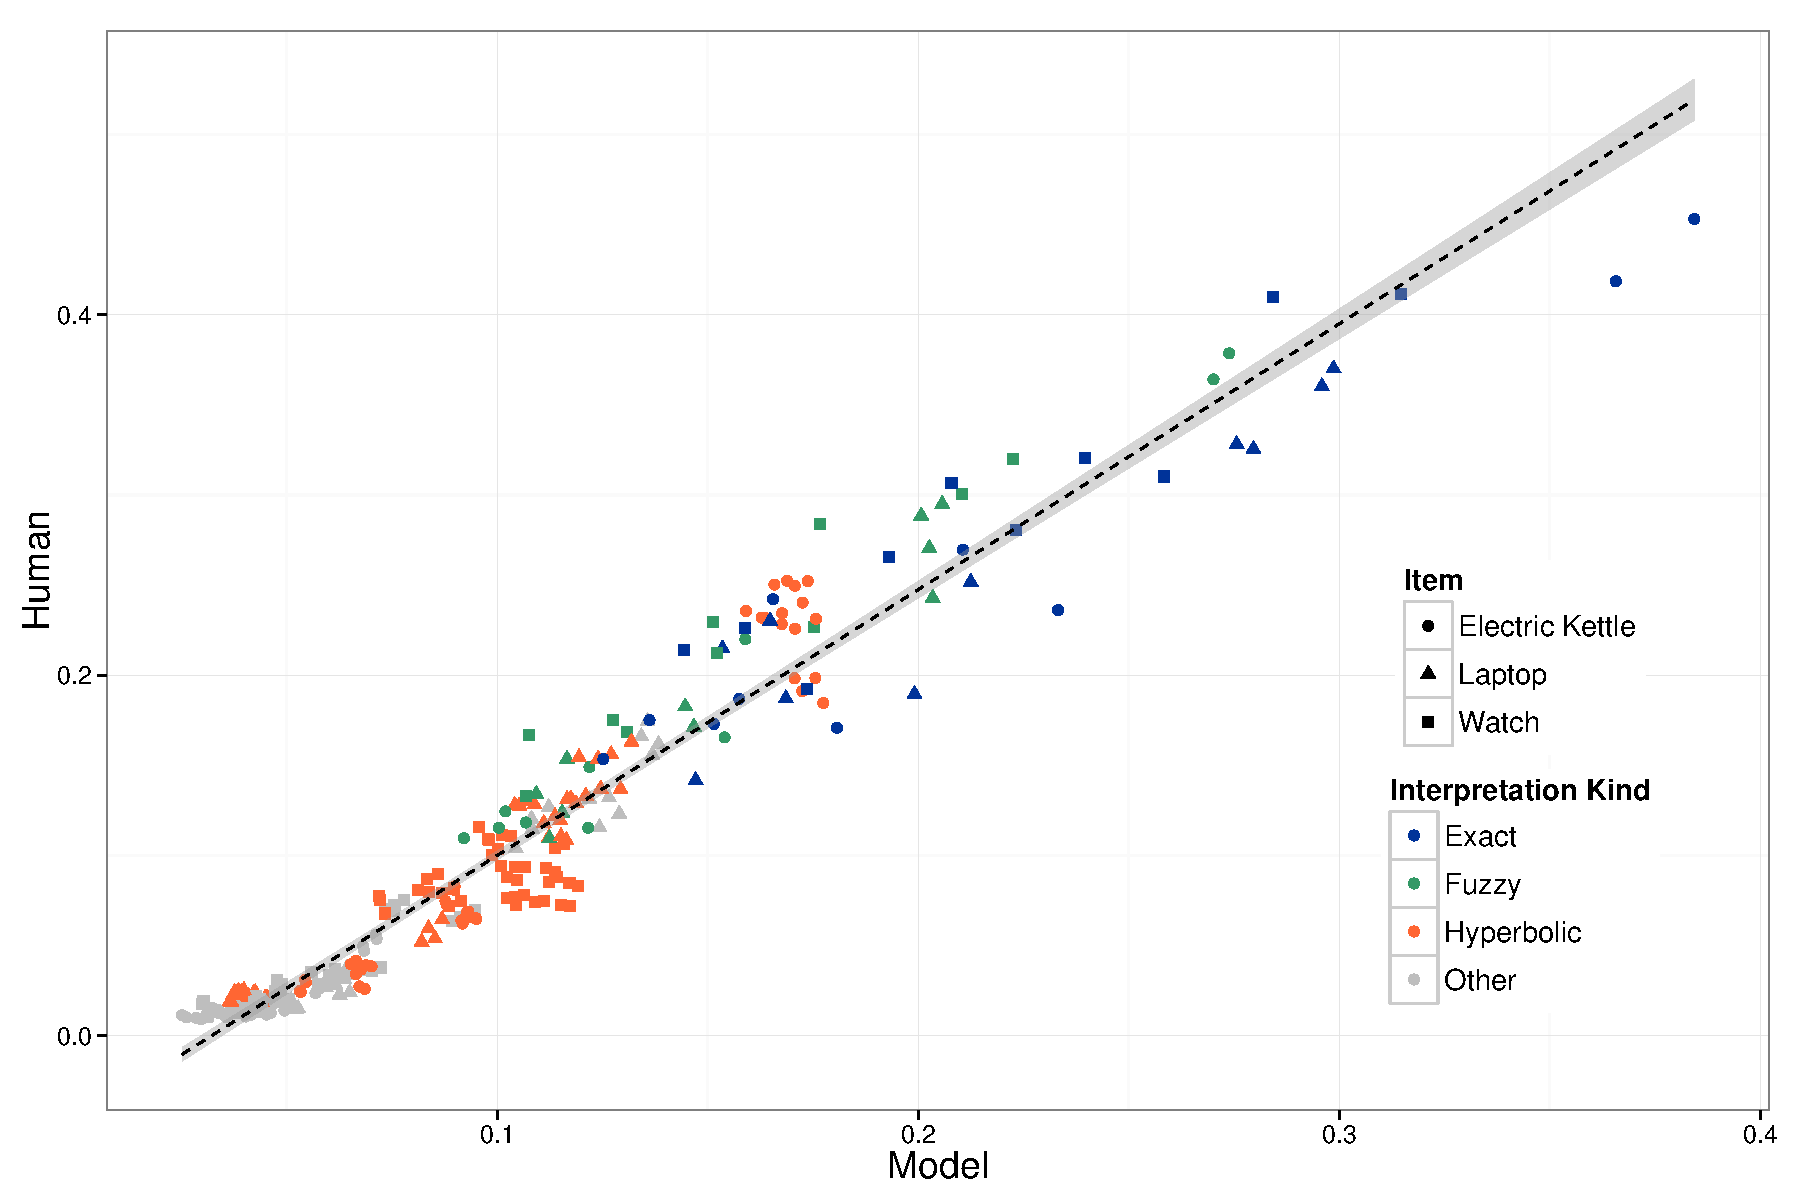
\includegraphics[width=8.7cm]{model_human_scatter.pdf}
\caption{Hello}\label{model_effects}
\end{minipage}\hfill
\begin{minipage}[b]{.49\textwidth}
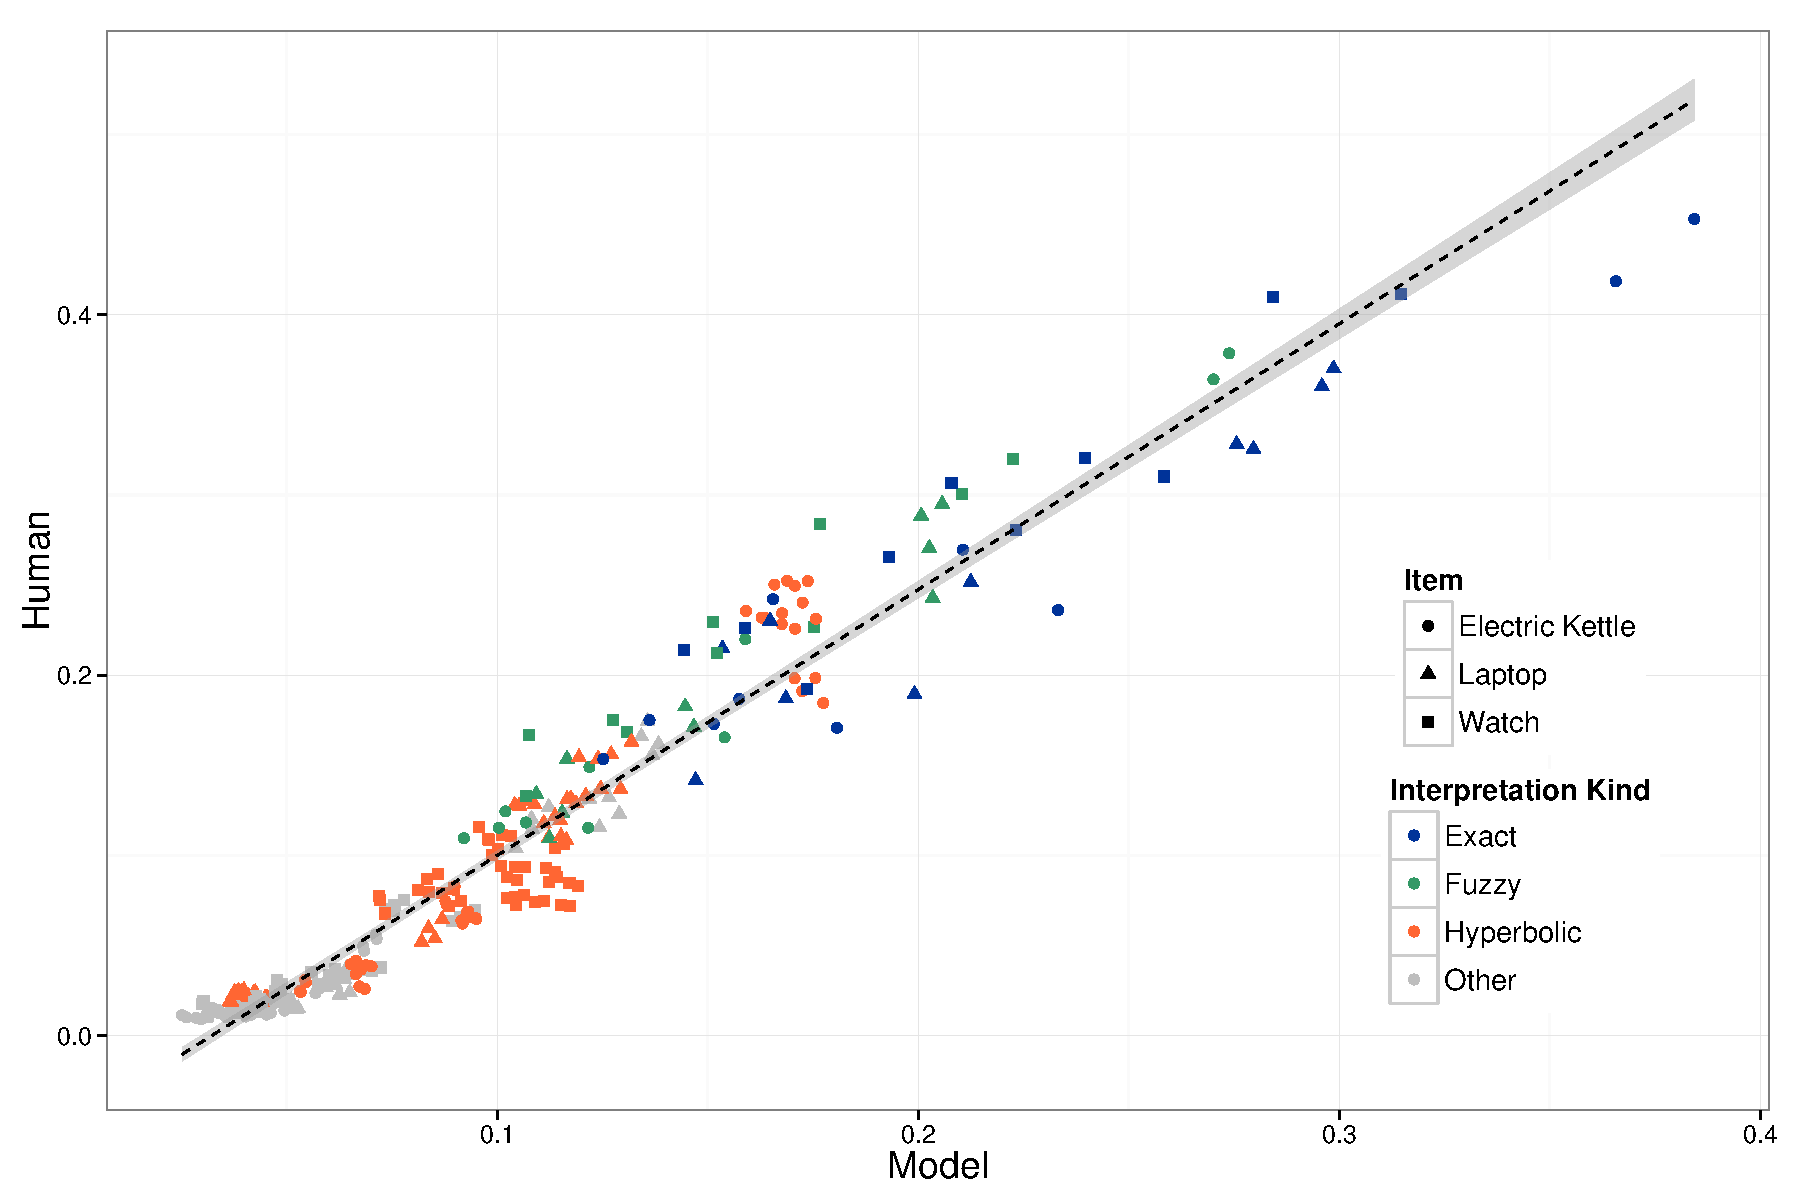
\includegraphics[width=8.7cm]{model_human_scatter.pdf}
\caption{Hello}\label{model_fit}
\end{minipage}
\caption{(a) This plot summarizes pragmatic halo, hyperbole, and affective interpretations of the model. (b) The model significantly predicts human interpretations with high correlation ($r=0.97$, $p<0.0001$) for all $300$ items.}
\end{figure*}

We test our model's interpretation of number expressions regarding the prices of three kinds of everyday items: \emph{electric kettles}, \emph{watches}, and \emph{laptops}. We focused on price because it is a common and natural topic of conversation in which people use number expressions. We chose the three items because they are common products whose price distributions are quite different from each other.
% QUESTION: Should we include a plot of scraped priors for these items to show that they're different?
We define the set of possible price states for the three kinds of items: $S=\{50, 50', 500, 500', 1000, 1000', 5000, 5000', 10000, 10000'\}$. Each price state is either ``round" (divisable by $10$) or ``sharp" (which we define as $n \pm k $, $k \in \{1, 2, 3\}$, where $n$ is round).
 We assume that the space of possible utterances $U$ is equivalent to the set of price states $S$. A speaker can say, ``That electric kettle cost $u$ dollars," for $u \in U$, and a listener can interpret this to mean that the kettle cost $s$ dollars, for $s \in S$.
 % FIXME: Notation might be confusing.
 
\subsection{Model simulations} 
%Our model considers the following five communicative goals: whether the speaker wants to convey the price precisely, imprecisely, or not at all, crossed with whether the speaker wants to convey her opinion about the price or not, minus the vacuous goal in which the speaker wants to convey nothing. We assume a uniform prior over goals. The model considers the possible price state meanings $S$ and the prior probability $P(s)$ of each price state for a given kind of item (see Experiment 2(a) in materials). It also considers the prior conditional probability $E(s)$ of a given price state being considered expensive (see Experiment 2(b) in materials). Finally, it considers the cost of each utterance $C(u)$ and assumes that sharp numbers are costlier to utter than round numbers. 

Given the formal setup of our model described in the methods section, we obtained posterior meaning distributions for the ten numerical utterances using the price priors and affect priors for each of the three items. Figure \ref{model_full_bar} in the Appendix shows the full meaning distribution for each utterance across the three item kinds. We seperated interpretations into three types: \emph{exact interpretations}, which are interpretations that are identical to the utterance (e.g. when``1000" is interpreted as meaning $1000$); \emph{fuzzy interpretations}, which are interpretations that are the sharp or round counterpart to the utterance (e.g. when ``1000" is interpreted as $1001$); and \emph{hyperbolic interpretations}, which are interpretations that are much smaller than the utterance (e.g. when ``1000" is interpreted as $50$ or $501$). The model also returns the probability of an utterance being interpreted as conveying \emph{affect} about the price being too expensive. Figure \ref{model_effects} summarizes these effects. We first see a basic effect of the prior, in which utterances that are more likely given the price prior of the item are more likely to be interpreted exactly or fuzzily (e.g. ``1000" is more likely to be interpreted exactly or fuzzily for laptops than for electric kettles). The model demonstrates the pragmatic halo effect, in which round utterances such as ``500" and ``1000" are interpreted less exactly and more fuzzily than their sharp counterparts ``501" and ``1001." It also demonstrates the hyperbole effect, in which utterances that are less likely given the price prior are more likely to be interpreted hyperbolically (e.g. ``1000" is more likely to be interpreted as $50, 51, 500,$ or $501$ for electric kettles than for laptops). We also see an interaction between halo and hyperbole, where round utterances such as ``5000" and ``10000" are more likely to be interpreted hyperbolically than their sharp counterparts. Furthermore, utterances whose literal meanings are associated with higher affect priors (such as ``10000" and ``10001") are more likely to be interpreted as conveying affect.

\begin{figure*}
\centering
\begin{minipage}[b]{.49\textwidth}
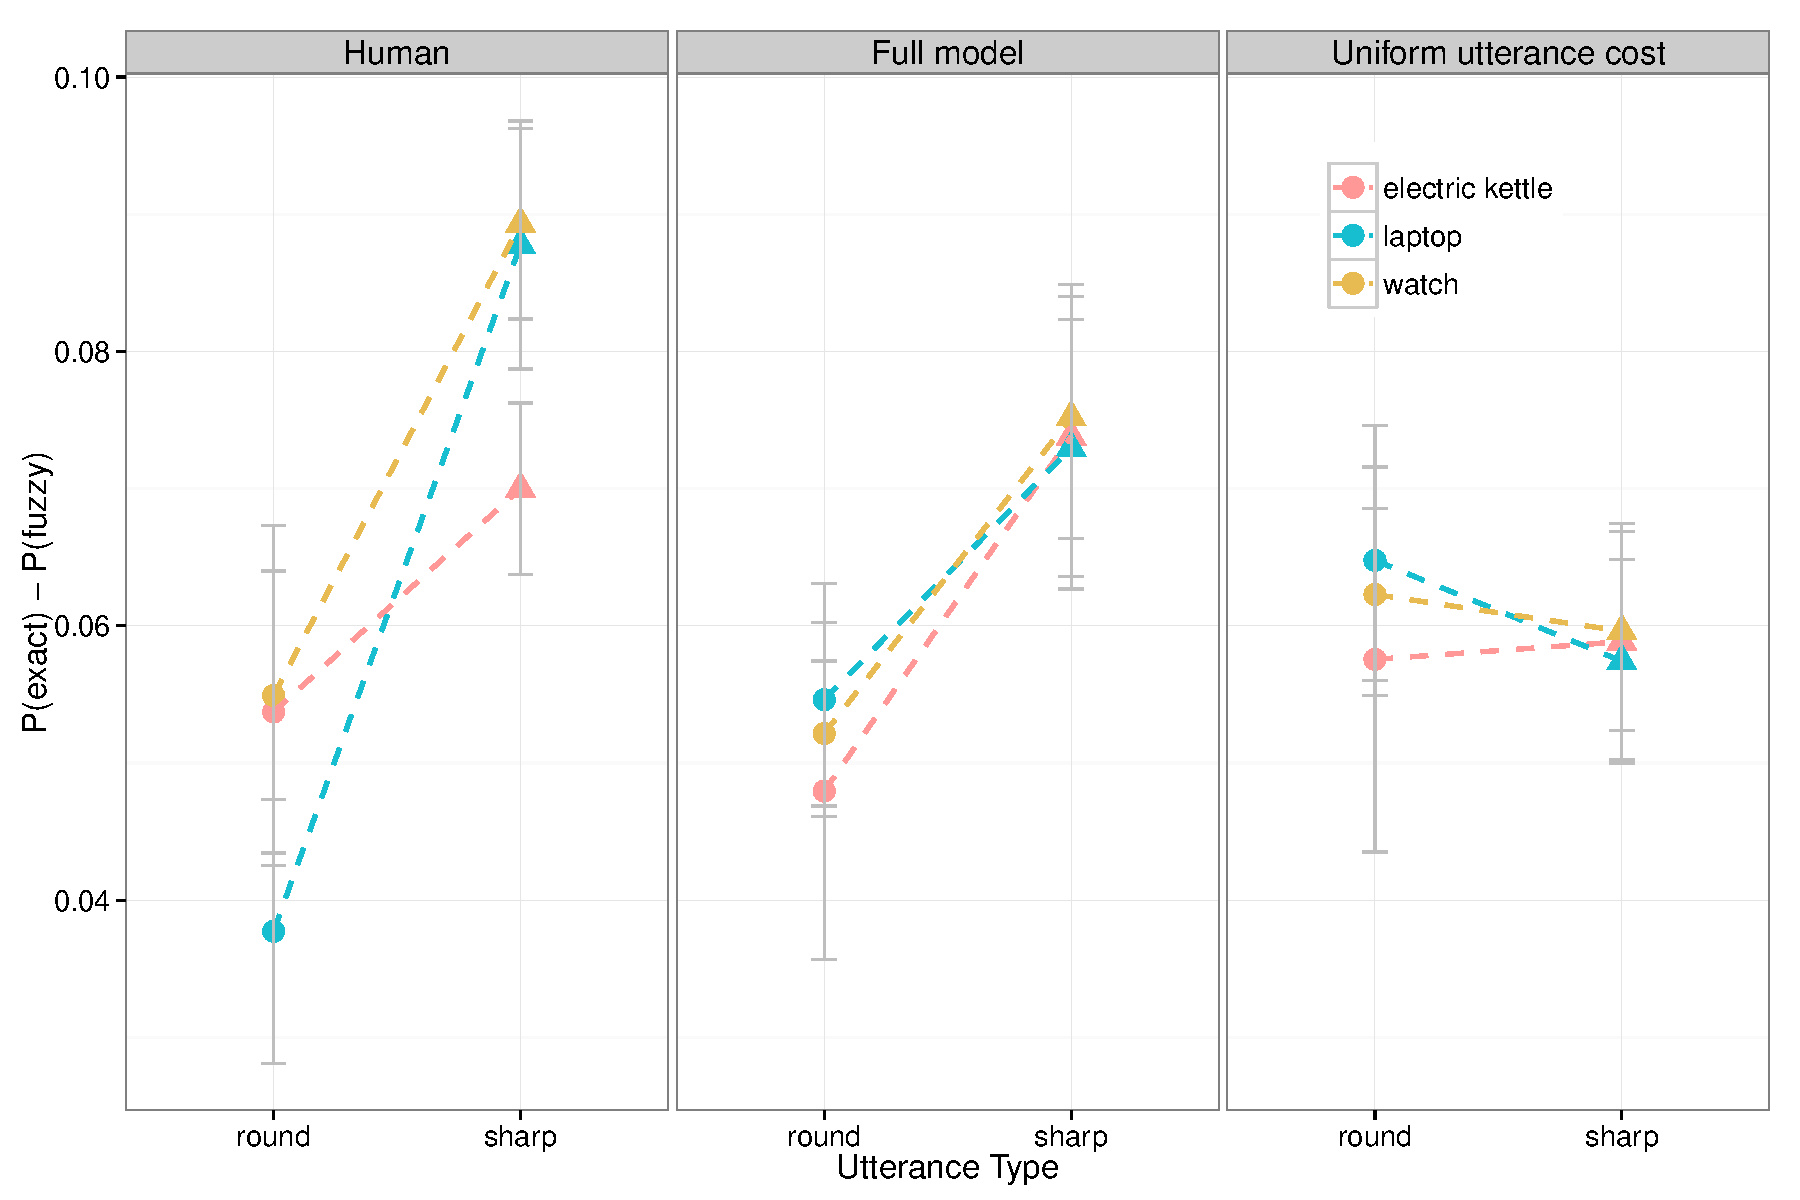
\includegraphics[width=8.7cm]{model_comp_halo.pdf}
\caption{Hello}\label{halo}
\end{minipage}\hfill
\begin{minipage}[b]{.49\textwidth}
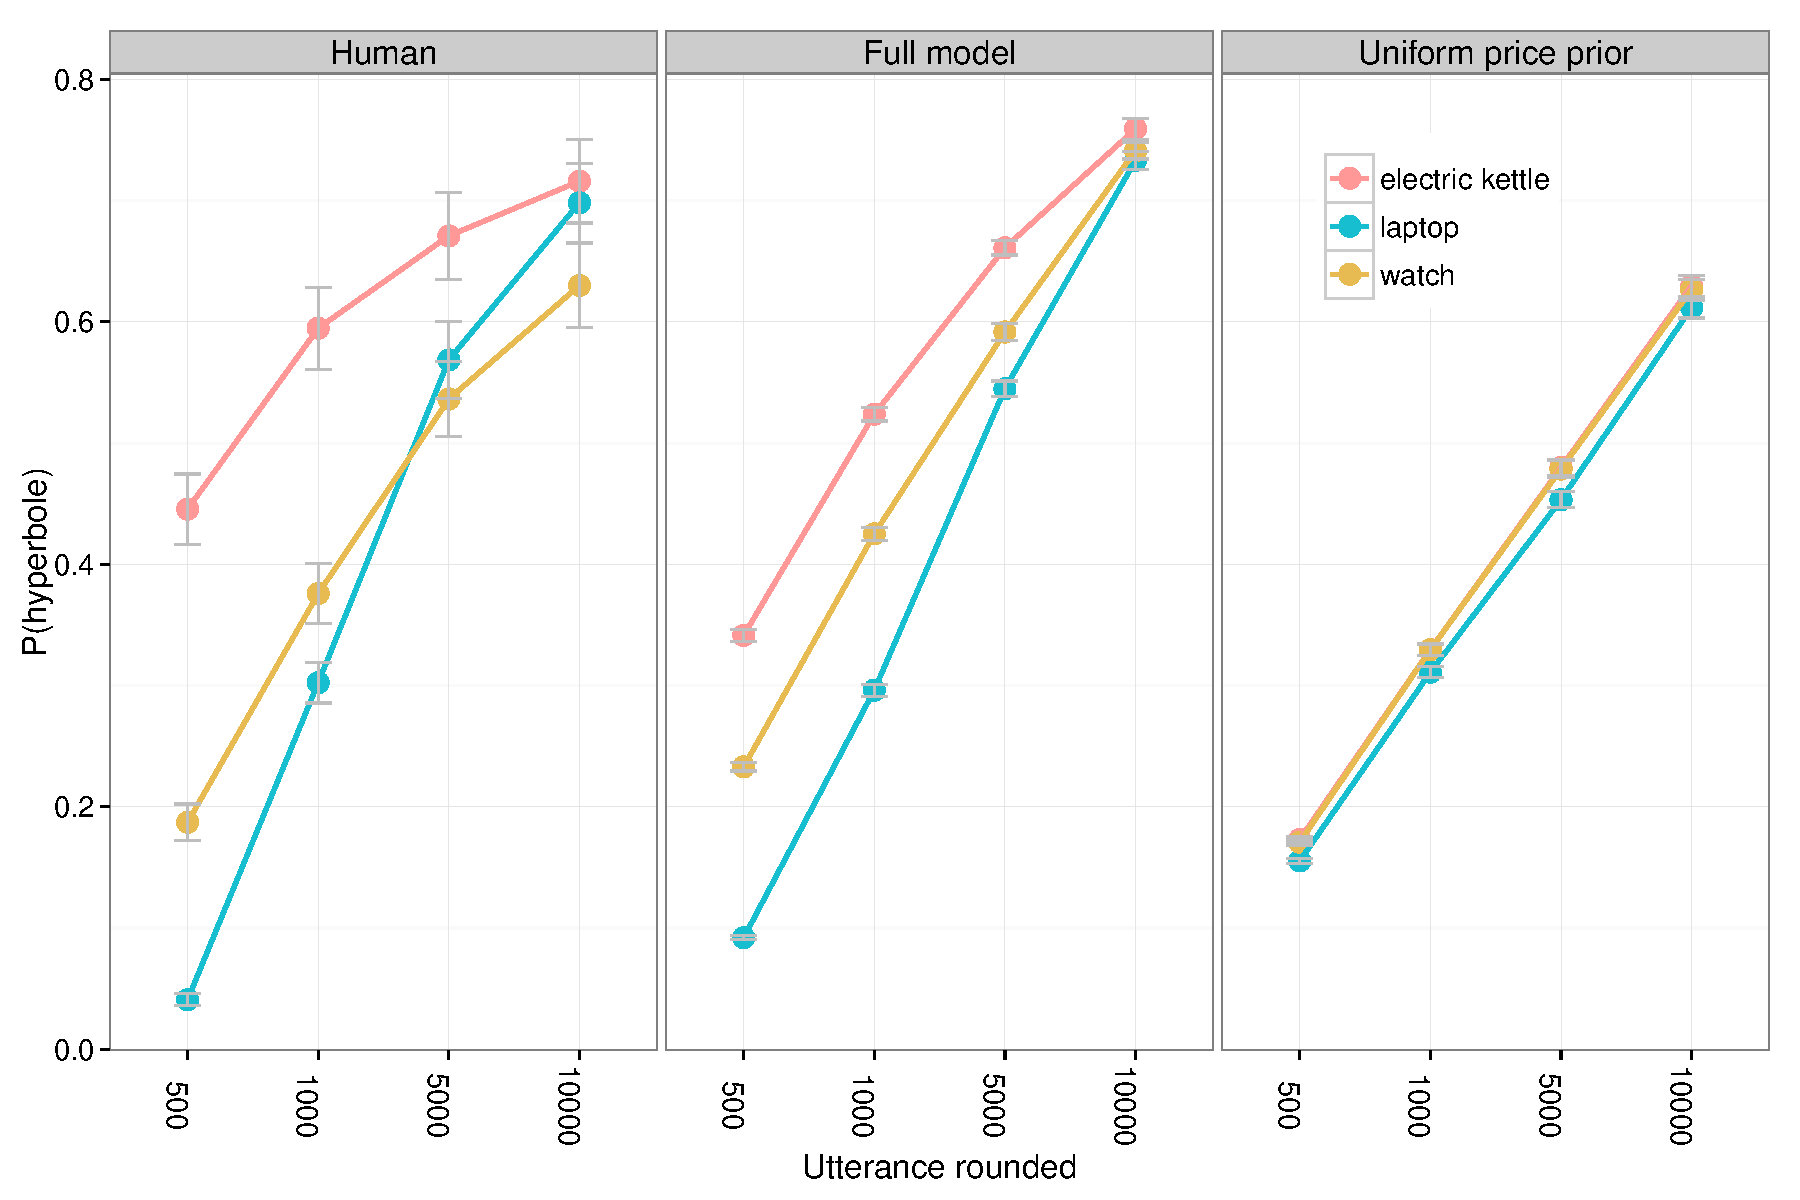
\includegraphics[width=8.7cm]{model_comp_hyperbole.pdf}
\caption{Hello}\label{hyperbole}
\end{minipage}
\caption{(a) Compares pragmatic halo. (b) Compares hyperbole. }
\end{figure*}

\begin{figure*}
\centering
\begin{minipage}[b]{.49\textwidth}
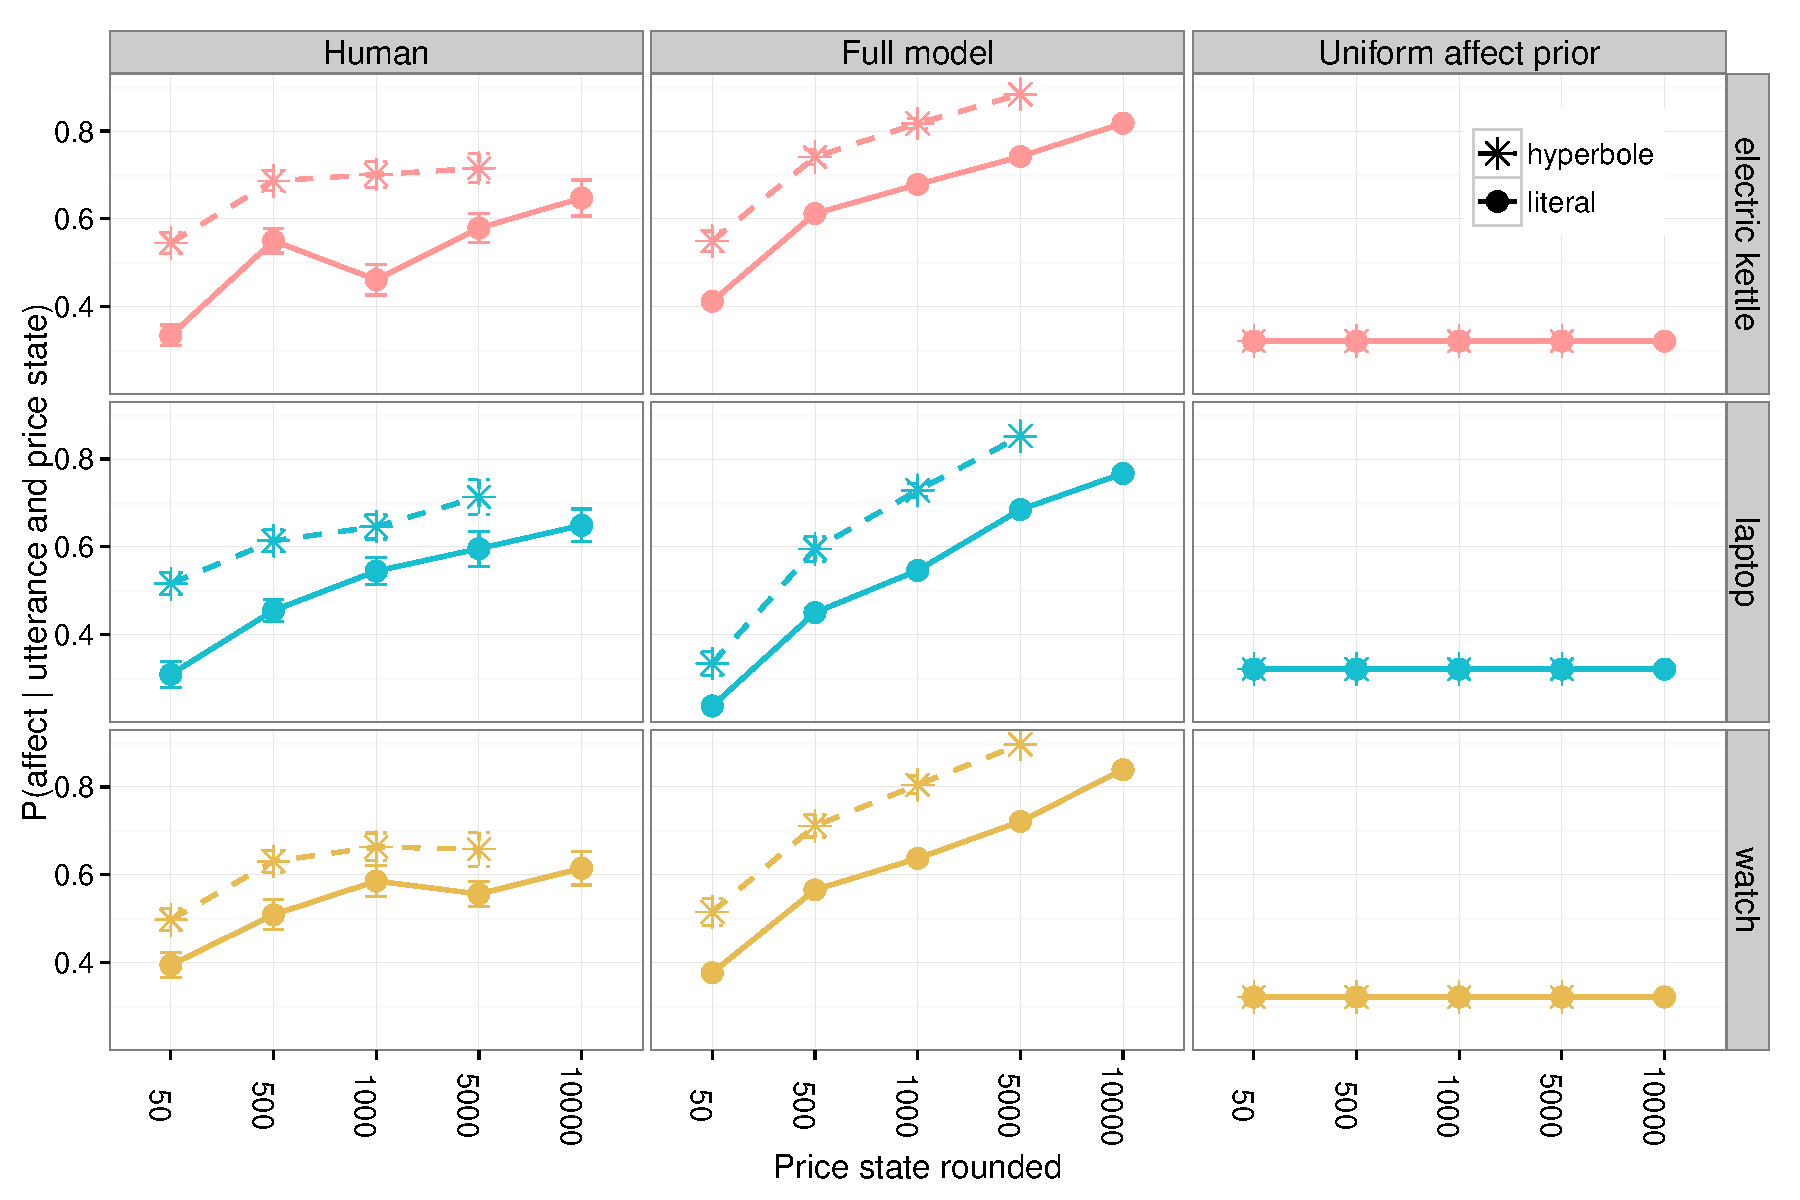
\includegraphics[width=8.7cm]{model_comp_affect.pdf}
\caption{Hello}\label{affect}
\end{minipage}\hfill
\begin{minipage}[b]{.49\textwidth}
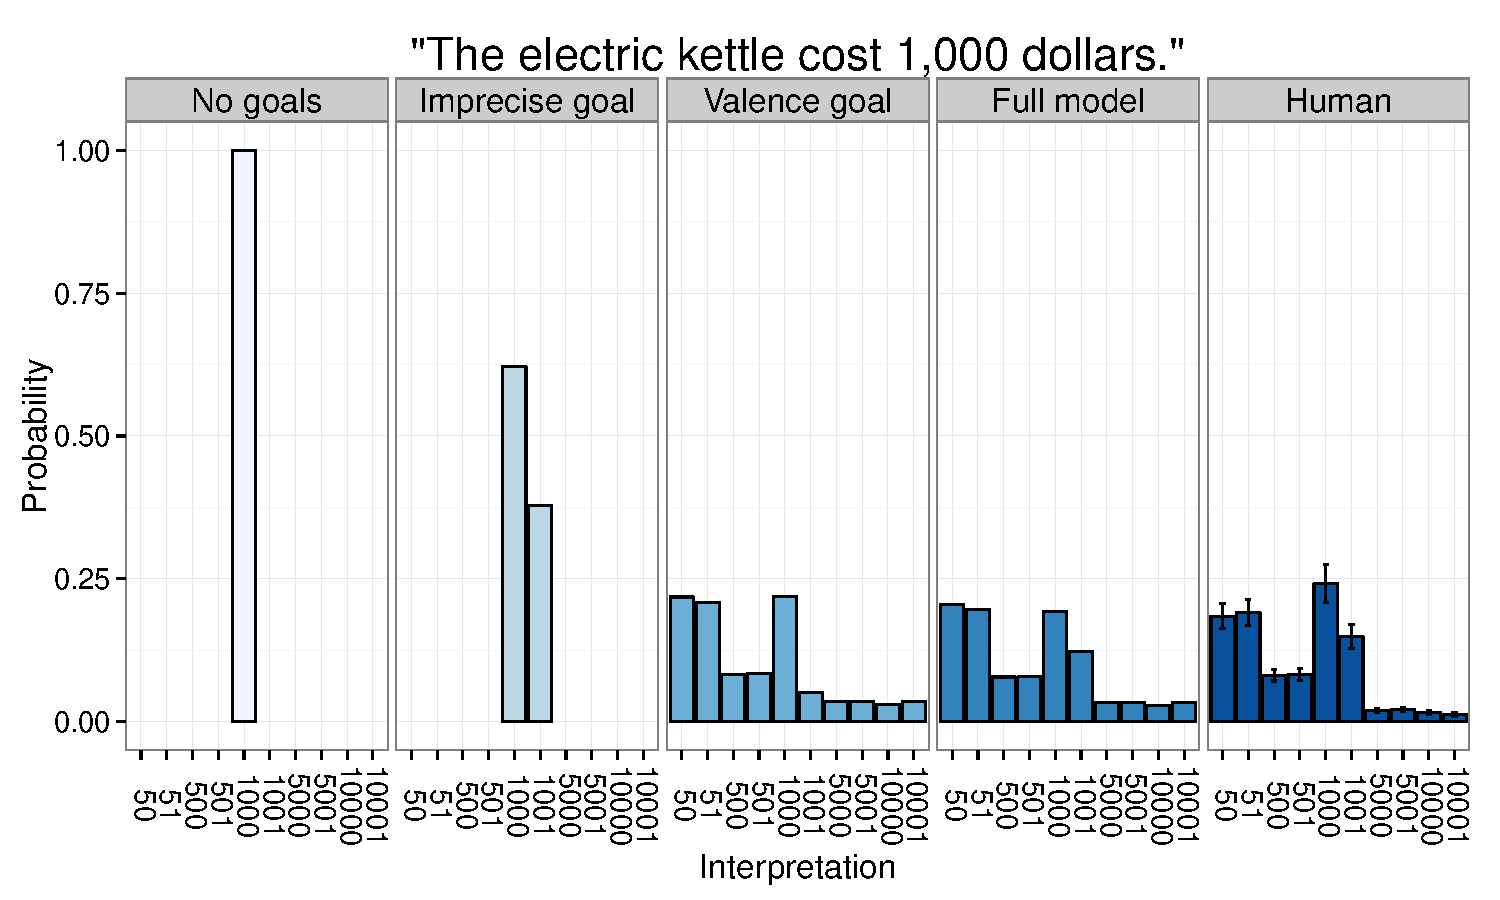
\includegraphics[width=8.7cm]{goals_comp.pdf}
\caption{Hello}\label{goals}
\end{minipage}
\caption{(a) Compares affective subtext. (b) Compares communicative goals.}
\end{figure*}

\subsection{Behavioral experiments}
Experiment 1a examined humans' interpretation of number words. We used the same set of items, price states $S$, and utterances $U$ as described earlier. Subjects read scenarios in which a buyer produces an utterance $u$ about the price of an item he just bought. Subjects rate the likelihood of the buyer thinking that the item was expensive, as well as the likelihood that the item actually cost $s$ dollars (see Experiment 1a in materials). Figure \ref{human_full_bar} in the Appendix shows the full interpretation distribution for each utterance. 

To examine the halo effect in humans, we computed the difference between the probability of an exact interpretation and the probability of a fuzzy interpretation for each utterance. Collapsed across items and utterances, this difference is significantly smaller for round numbers than for sharp numbers ($F(1, 4)=16.31,  p < 0.05)$, which indicates that round numbers tend to be interpreted more approximately and have a weaker bias towards exact interpretation than their sharp counterparts. To examine the hyperbole effect, we show that utterances whose literal meanings have low probabilities under the item's prior price distribution are more likely to be interpreted hyperbolically ($F(1, 10) = 44.06, p < 0.0001$).

Experiment 1b examined the affective subtext conveyed using hyperbolic versus literal utterances. Subjects read scenarios in which a speaker bought an item that cost $s$ dollars and tells his friend that it cost $u$ dollars, where $u >= s$. Subjects rate the likelihood of the buyer thinking that the item was expensive (see Experiment 1b in materials). Results showed that utterances $u$ where $u > s$ are rated as significantly more likely to convey affect than utterances where $u = s$ ($F(1, 25) = 9.592, p < 0.01)$, confirming the hypothesis that listeners infer affective subtext from hyperbolic utterances.
%We broke down the interpretations into \emph{exact}, \emph{fuzzy}, and \emph{hyperbolic}. Figure \ref{human_effects} summarizes these effects. We see that round utterances tend to be interpreted less exactly and more fuzzily than their sharp counterparts, and utterances that are less likely given the price prior are more likely to be interpreted hyperbolically. We also see that round utterances are more likely to be interpreted hyperbolically.
%%TODO
% Figure out what stats to report here.

\subsection{Comparison}
We compared model and human interpretation probabilities for the $300$ items ($I \times U \times S$) and show that model predictions correlate significantly with human interpretations of number words ($r=0.968$, $p<0.0001$) (Figure \ref{model_fit}). We also show that each component of the model is responsible for capturing the effects that we observe in the human data. 

% Fix figure numbers
The left-most panel in Figure 3 shows the halo effect in humans, namely the tendency for round numbers to be interpreted less exactly. This effect is replicated by the full model, but not by a version of the model where the costs of utterances are uniform. This suggests that people take into account utterance cost when inferring exact versus fuzzy interpretations. The leftmost panel in Figure 4 shows humans' probabilities of interpreting each utterance hyperbolically. These probabilities are captured faithfully by the full model, but not by a version of the model where the price prior distribution for each item is uniform. This suggests that people take into account the prior distribution of prices when inferring hyperbolic versus literal interpretations. 

The leftmost panels in Figure 5 show humans' probabilities of inferring affective subtext given a price state and a literal or hyperbolic utterance. Within the same price state, hyperbolic utterances are interpreted as conveying more affect than literal utterances. Across price states, higher price states are associated with higher degrees of affect. Both effects are replicated by the full model, but not by a version of the model where the probability of affect given each price state is uniform. This suggests that the affective subtext conveyed by hyperbolic utterances is driven by prior probabilities of affect given a price state. Moreover, utterances interpreted hyperbolically convey affective subtext beyond the prior affect associated with the actual state of the world. 

Finally, we show that reasoning about a speaker's communicative goals is crucial for capturing the non-literal interpretation of number words demonstrated in the behavioral experiment. Figure 6 compares different model interpretations of the utterance \emph{``The electric kettle cost $1000$ dollars."} A listener that does not consider alternative communicative goals interprets the utterance literally and places all interpretation mass on the price state $1000$. A listener that considers a speaker whose goal may be to communicate precisely or imprecisely places a significant amount of interpretation mass on the neighboring price state $1001$. A listener that considers a speaker whose goal may be to communicate the precise price state or her affect about the price state can now interpret the utterance hyperbolically and place mass on price states with higher prior probabilities. However, he places very little mass on the neighboring price state $1001$. Finally, a listener that considers the possibility of precise, imprecise, and affect goals closely fits humans' interpretation of the utterance.
%------------------------------------------------
\section{Discussion}
%Despite having highly standard literal meanings, numbers are often used non-literally in everyday language. 
Our model and behavioral results reveal complex patterns in the non-literal interpretation of number words. We show that these patterns depend on the listener's prior knowledge, consideration of communication efficiency, and reasoning about the speaker's communicative goal. Besides producing quantitative predictions for pragmatic number interpretation, we also introduce an ``affect" dimension that takes into account social and subjective aspects of communication.  Our model shows that rational recursive reasoning between speaker and listener can capture rich effects in language understanding that have been difficult to model formally. We present an innovative formal framework for examining phenomena in non-literal language understanding, and provide evidence that this framework and its extensions will advance language research such that some day--hyperbolically speaking--Bayesian models can explain ``\emph{everything}."


%----------------------------------------------------------------------------------------
%	MATERIALS AND METHODS
%----------------------------------------------------------------------------------------

%% Optional Materials and Methods Section
%% The Materials and Methods section header will be added automatically.

\begin{materials}
\section{Model}
Here we describe our model in detail. Let $u$ be the utterance a speaker utters. Let $m$ be the meaning that is known to the speaker. $m$ has two dimensions, one concerning the actual price state $s$, and one concerning the speaker's affect $a$. Given the set of price states $S$ and set of affect states $A$, the set of possible meanings $M$ is given by $M = S \times A$. We denote each possible meaning as $m_{s,a}$, where $s \in S$ and $a \in A=\{0, 1\}$ ($0$ means no affect and $1$ means with affect). 

Let $g$ be the communicative goal, which also has two dimensions, one concerning the price state, and the other concerning the speaker's affect. We denote each communicative goal as $g_{\mathbf{s},\mathbf{a}}$ where $\mathbf{s} \in 2^{S}$ and $\mathbf{a} \in 2^{A}$. The goal $g_{\mathbf{s},\mathbf{a}}$ is a function $g_{\mathbf{s},\mathbf{a}}: M \rightarrow \{0,1\}$, such that $g_{\mathbf{s},\mathbf{a}}(m_{s,a})=1$ if and only if $s \in \mathbf{s}, a \in \mathbf{a}$. Thus, a goal specifies a subset of price states and affects, and a meaning satisfies this goal if it belongs to this subset; such a subset will be referred to as a goal state. We assume that there are two types of price-related goal states: the speaker either wants to communicate the price state exactly or approximately. Exact goals are represented by subsets that consist of a single price state, i.e. $\mathbf{s}=\{i\}$ (for some $i \in S$), and approximate goals are represented by subsets that consist of the price states within a distance of 1 of some state, i.e. $\mathbf{s}=\{j | j \in S, |j-i|\leq 1\}$. 

The prior probability of a price state $s$ is taken from an empirically derived price prior $P_S(s)$, and the probability of an affect $a$ given a price state $s$ is taken from an empirically derived conditional affect prior $P_A(a|s)$ (see Experiments 2a and 2b). The probability distribution $P_G(\cdot|m_{s,a})$ over goals given that teh speaker knows meaning $m_{s,a}$ is defined to be uniform over goals consistent with $m_{s,a}$, i.e. uniform over goals $g_{\mathbf{s},\mathbf{a}}$ such that $g_{\mathbf{s},\mathbf{a}}(m_{s,a})=1$. This is equivalent to assuming that the speaker either wants to communicate their meaning exactly or approximately.

A literal listener $L_0$ provides the base case for recursive social reasoning between the speaker and listener. $L_0$ interprets an utterance $u$ literally without taking into account the speaker's communicative goals:

%\begin{equation}\label{eq:literallistener}
%\text{
\[ L_0(m_{s,a} |u) = \left\{ 
  \begin{array}{l l}
    P_A(a|s) & \quad \text{if $s$ = $u$}\\
    0 & \quad \text{otherwise}
  \end{array} \right.\]
 % }
%\end{equation}

The speaker $S_n$ is assumed to be a rational planner who optimizes the probability that the listener will infer a meaning $m$ that satisfies her communicative goal while minimizing the cost of her utterance. $S_n$ chooses utterances according to a softmax decision rule that describes an approximately rational planner \cite{sutton1998reinforcement}:
\begin{equation}\label{eq:speakerprob}
S_n(u | g_{\mathbf{s},\mathbf{a}}) \propto e^{\lambda U_n(u |  g_{\mathbf{s},\mathbf{a}})}
\end{equation}
where the constant $\lambda$ captures the degree of optimality of the speaker. (We used $\lambda=1$ in the model simulations described).
The speaker wants to minimize both the cost $C(u)$ of the utterance and the surprisal of her goal state. The utility function $U_n$ is therefore defined by:
\begin{equation}
U_n(u |  g_{\mathbf{s},\mathbf{a}}) = \log (P(g_{\mathbf{s},\mathbf{a}}(L_n(m|u)) =1) - C(u)
\end{equation}
which combined with equation \ref{eq:speakerprob} leads to:
\begin{equation}\label{eq:speakersimplified}
S_n(u | m, g) \propto (P(g_{\mathbf{s},\mathbf{a}}(L_n(m|u)) =1)\cdot e^{-c(u)}) ^\lambda.
\end{equation}

The listener $L_n$ performs Bayesian inference to guess the intended meaning given the prior $P$ and his internal model of the speaker. To determine the speaker's intended meaning, the listener will marginalize over the possible goals under consideration.

\begin{equation}\label{eq:listenerdict}
L_n(m_{s,a}|u) \propto \sum_{g }P_S(s)P_A(a|s)P_G(g|m_{s,a})S_{n-1}(u | g).
\end{equation}

After obtaining a posterior distribution for all possible meanings $m$ given an utterance $u$, we performed a Luce choice transformation on the distribution with $\lambda = 0.5$ in order to compare with behavioral results.

\section{Experiment 1a: Halo and hyperbole}
$120$ subjects were recruited on Amazon's Mechanical Turk. Each subject read $15$ scenarios in which a person (e.g. Bob) buys an item (e.g. a watch) and is asked by a friend whether the item is expensive. Bob responds by saying ``It cost $u$ dollars," where $u \in \{50, 50\pm k, 500, 500\pm k, 1000, 1000 \pm k, 5000, 5000 \pm k, 10000, 10000 \pm k\}$, where $k$ was randomly selected from the set $\{1, 2, 3\}$ for each trial. We will refer to this set of utterances as $U$. Given an utterance $u$, subjects rated the probability of Bob thinking that the item was expensive. They then rated the probability of the item costing the following amounts of money: $50$, $50\pm k$, $500$, $500\pm k$, $1000$, $1000 \pm k$, $5000$, $5000 \pm k$, $10000$, $10000 \pm k$, where $k$ was randomly selected from the set $\{1, 2, 3\}$ for each trial. We will refer to this set of prices as $S$. Ratings for each price state were on a continuous scale from ``impossible" to ``extremely likely", represented as real values between $0$ and $1$. We normalized subjects' ratings across price points for each trial to sum up to $1$. The average normalized ratings across subjects for each item/utterance pair is shown in Figure \ref{human_full_bar}.

\section{Experiment 1b: Affective subtext}
$160$ subjects were recruited on Amazon's Mechanical Turk. Each subject read $30$ scenarios in which a person (e.g. Bob) buys an item that costs $s$ dollars and is asked by a friend whether the item is expensive. Bob responds by saying ``It cost $u$ dollars," where $u \in U$ and $u >= s$. Subjects then rated how likely Bob thinks the item was expensive on a continuous scale ranging from ``impossible" to "absolutely certain," represented as real values between $0$ and $1$. The average ratings determine the degree of affect conveyed by an utterance given the actual price state.

\section{Experiment 2a: Price prior}
To obtain people's prior knowledge of the price distributions for electric kettles, laptops, and watches, $30$ subjects were recruited from Amazon's Mechanical Turk. Each subject rated the probability of an electric kettle, laptop, and watch costing $s$ dollars, where $s \in S$ (see Experiment 1a). Ratings for each price state were on a continuous scale from ``impossible" to ``Extremely likely", represented as real values between $0$ and $1$. We normalized subjects' ratings across price points for each trial to sum up to $1$. The average normalized ratings across subjects for each item were taken as the prior probability distribution of item prices. These price distributions were used in the model to determine the prior probability of each price state.

\section{Experiment 2b: Affect prior}
To obtain people's prior knowledge of the affect likelihood given a price state, $30$ subjects were recruited from Amazon's Mechanical Turk. Each subject read $15$ scenarios where someone had just bought an item that cost $s$ dollars ($s \in S$). They then rated how likely the buyer thinks the item was expensive on a continuous scale ranging from ``impossible" to "absolutely certain," represented as real values between $0$ and $1$. The average ratings for each item/price state pair were taken as the prior probability of an affect given a price state. This was used in the model to determine the prior probability of an affect given each price state.

\end{materials}

%----------------------------------------------------------------------------------------
%	APPENDICES (OPTIONAL)
%----------------------------------------------------------------------------------------

\appendix[Appendix title]
\begin{figure*}[h]
\centering
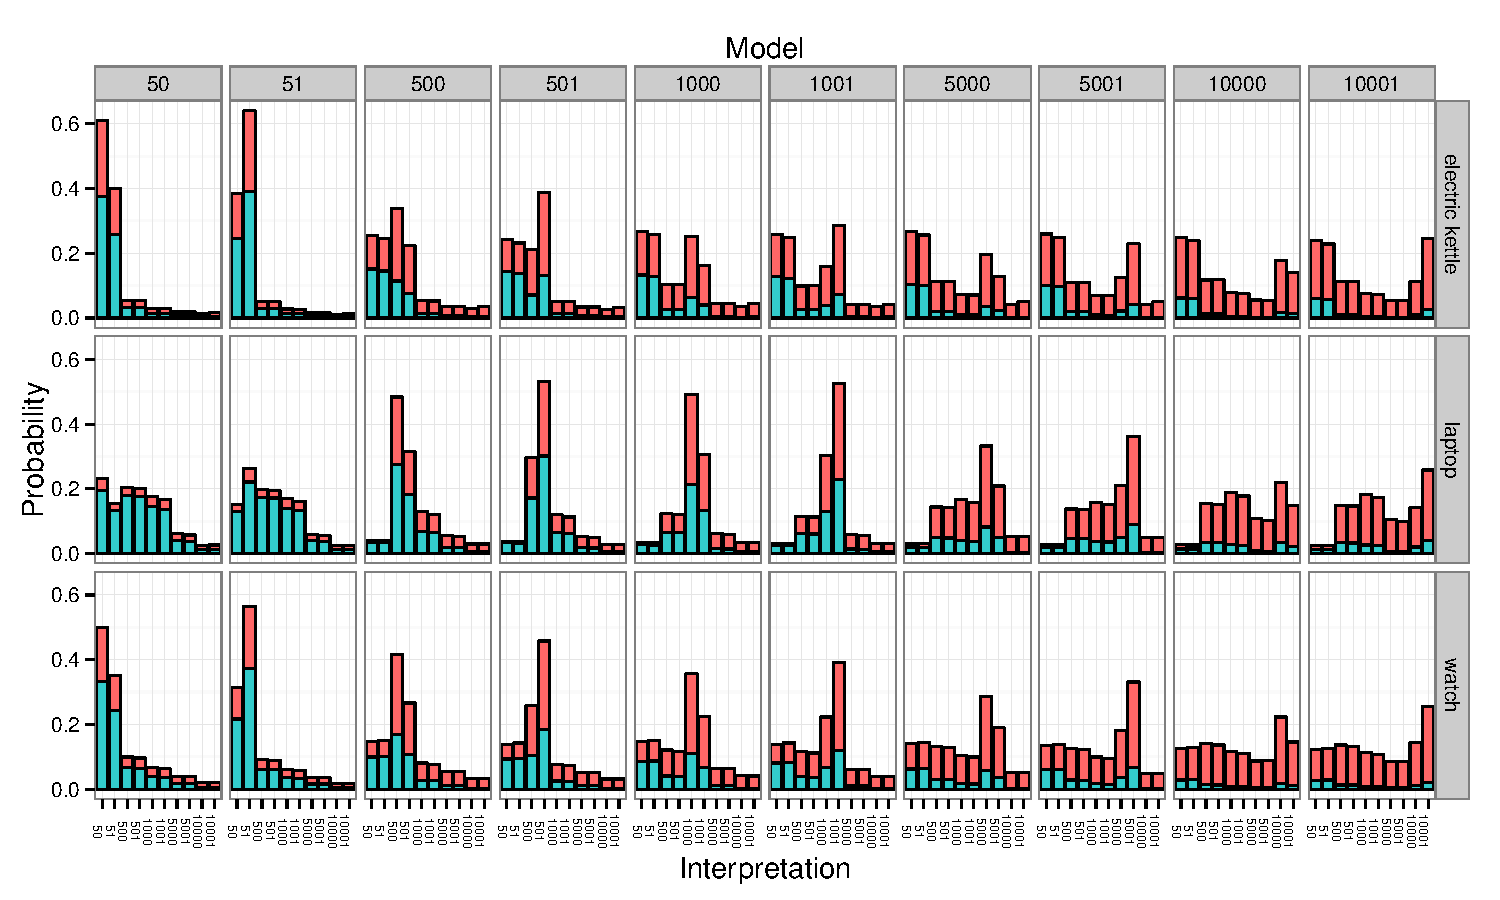
\includegraphics[width=16cm]{model_full_bar.pdf}
\caption{Hello}\label{model_full_bar}
\end{figure*}
\begin{figure*}
\centering
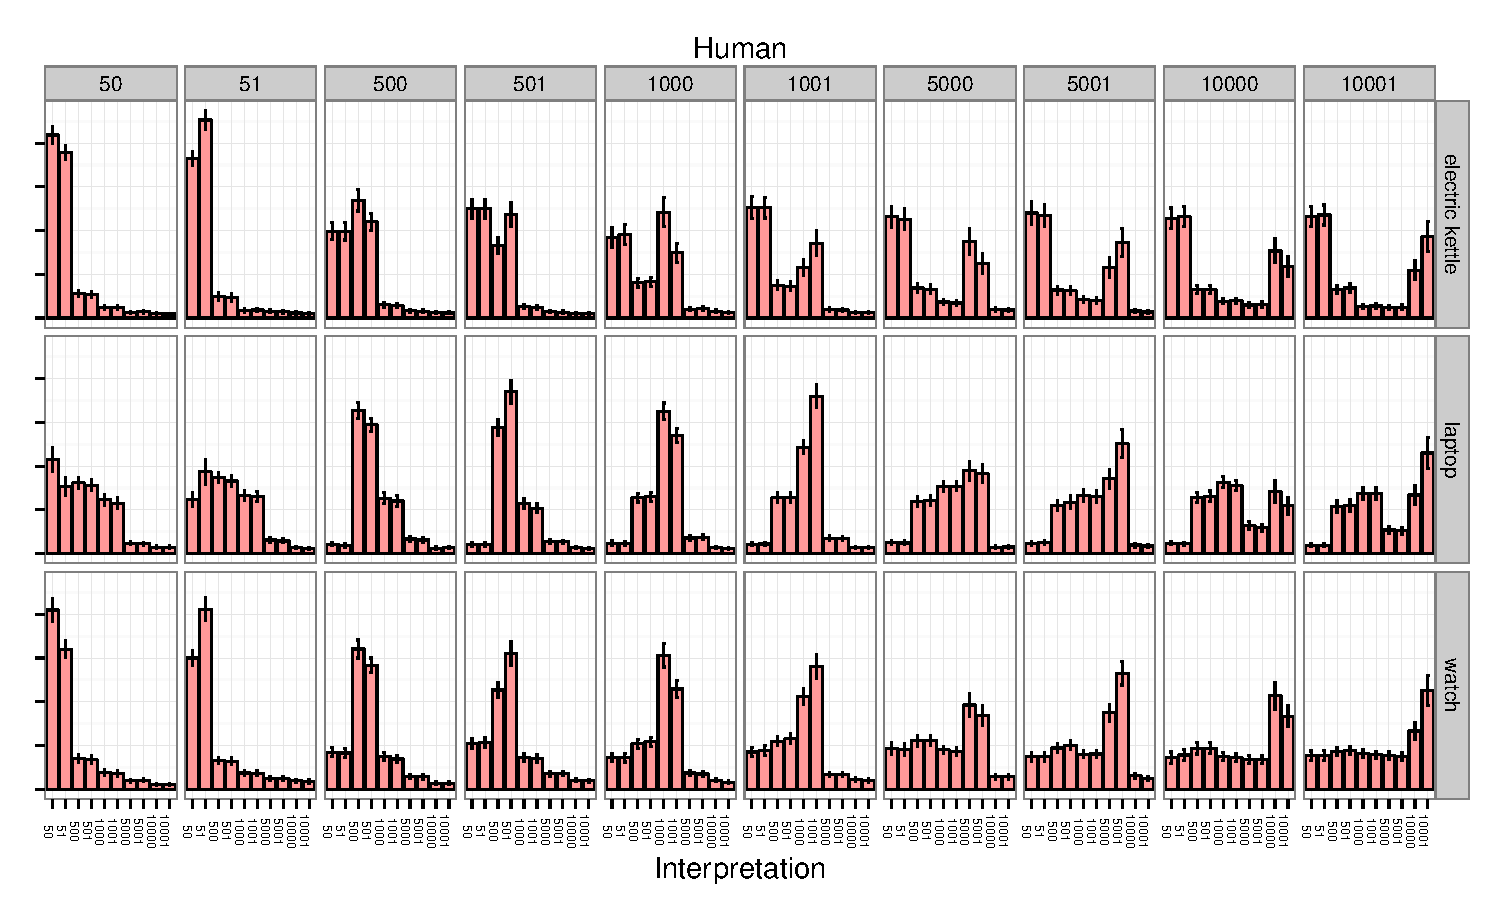
\includegraphics[width=16cm]{human_full_bar.pdf}
\caption{Hello}\label{human_full_bar}
\end{figure*}
%\begin{figure*}[h]
%\centering
%\begin{minipage}[b]{.49\textwidth}
%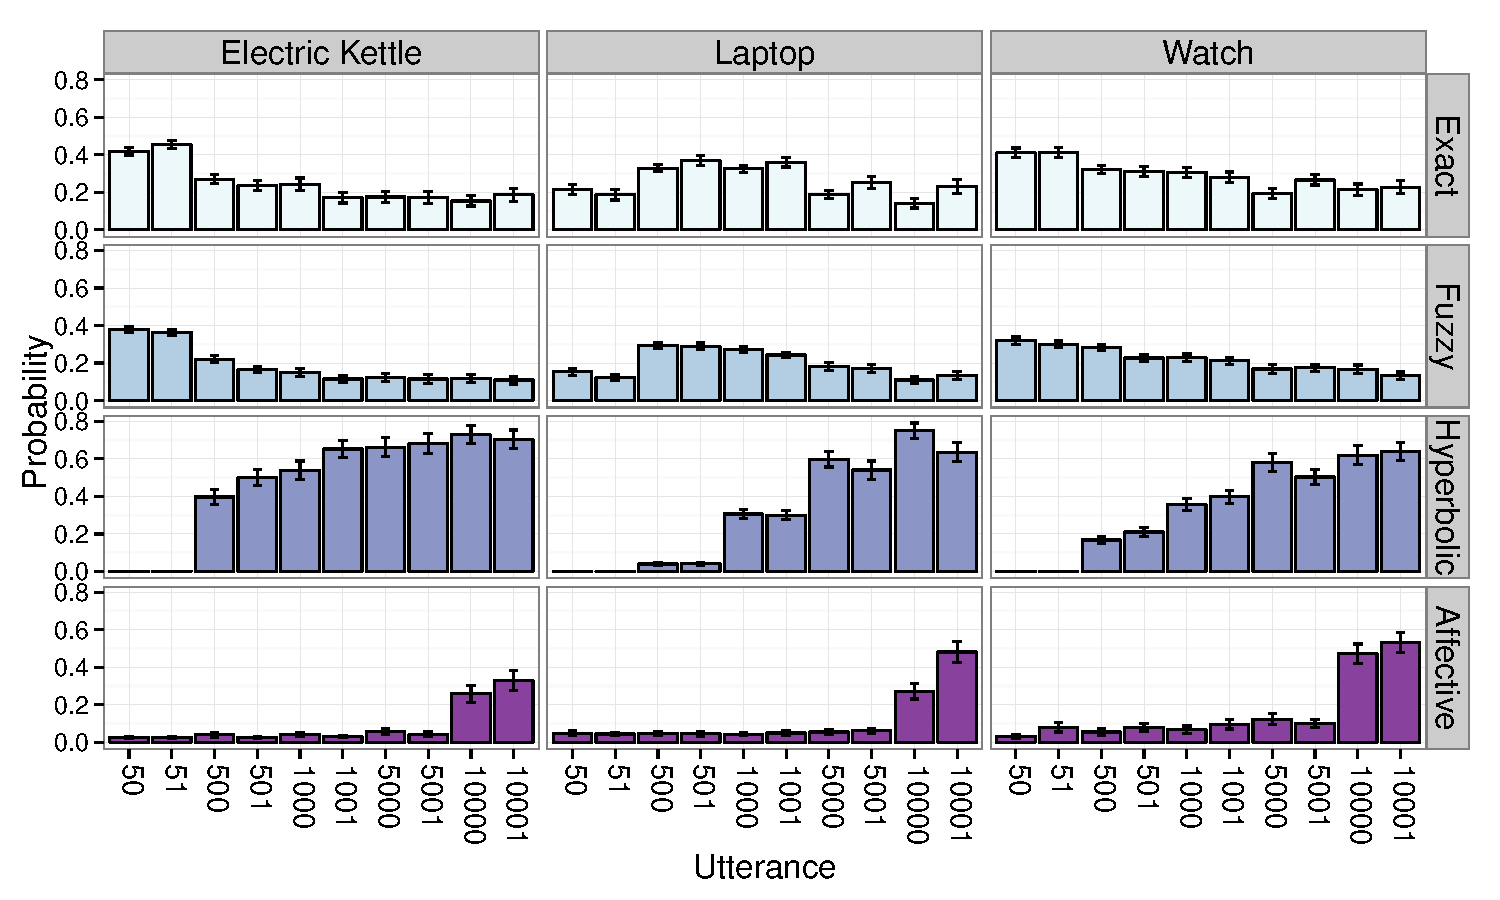
\includegraphics[width=8.7cm]{human_effect_bar.pdf}
%\caption{Hello}\label{model_effects}
%\end{minipage}\hfill
%\begin{minipage}[b]{.49\textwidth}
%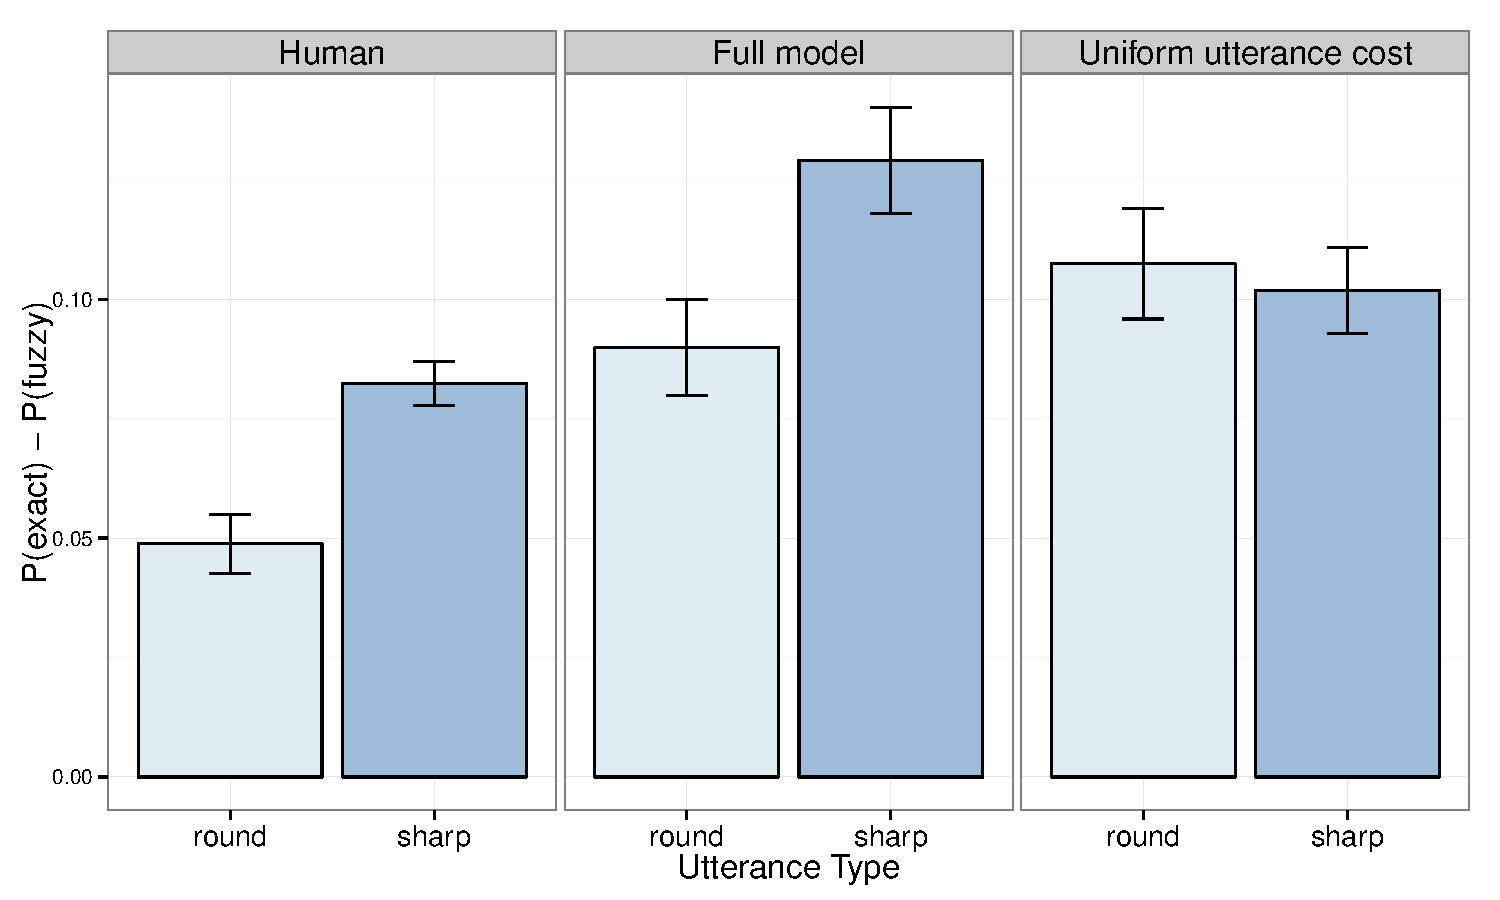
\includegraphics[width=8.7cm]{halo_comp.pdf}
%\caption{Vertical panels show results for the three item kinds. Horizontal panels show the three kinds of interpretations, \emph{exact}, \emph{fuzzy}, and \emph{hyperbolic}. The $x$ axis in each panel represents the utterance. The $y$ axis shows the probability of a kind of interpretation given the utterance.}\label{human_effects}
%\end{minipage}
%\end{figure*}

%%%%
% QUESTION: Not sure if we want this table....
%%%
%\begin{table}
%\begin{tabular}{l l}
%\hline
%\textbf{Model} & \textbf{Fit ($R^2$)}\\
%\hline
%Full & $0.938$\\
%Uniform prior & 0.560 \\
%Uniform cost & 0.939 \\
%Uniform affect & 0.921 \\
%No valence goal & 0.144 \\
%No imprecision goal & 0.726 \\
%\hline
%\end{tabular}
%\label{model_fit}
%\end{table}


%----------------------------------------------------------------------------------------
%	ACKNOWLEDGEMENTS
%----------------------------------------------------------------------------------------

\begin{acknowledgments}
Thanks!
\end{acknowledgments}

%----------------------------------------------------------------------------------------
%	BIBLIOGRAPHY
%----------------------------------------------------------------------------------------

%% PNAS does not support submission of supporting .tex files such as BibTeX.
%% Instead all references must be included in the article .tex document. 
%% If you currently use BibTeX, your bibliography is formed because the 
%% command \verb+\bibliography{}+ brings the <filename>.bbl file into your
%% .tex document. To conform to PNAS requirements, copy the reference listings
%% from your .bbl file and add them to the article .tex file, using the
%% bibliography environment described above.  

%%  Contact pnas@nas.edu if you need assistance with your
%%  bibliography.

% Sample bibliography item in PNAS format:
%% \bibitem{in-text reference} comma-separated author names up to 5,
%% for more than 5 authors use first author last name et al. (year published)
%% article title  {\it Journal Name} volume #: start page-end page.
%% ie,
% \bibitem{Neuhaus} Neuhaus J-M, Sitcher L, Meins F, Jr, Boller T (1991) 
% A short C-terminal sequence is necessary and sufficient for the
% targeting of chitinases to the plant vacuole. 
% {\it Proc Natl Acad Sci USA} 88:10362-10366.


%% Enter the largest bibliography number in the facing curly brackets
%% following \begin{thebibliography}

\begin{thebibliography}{10}

%\bibitem{moreno2007creativity}
%Moreno, R.E.V.,
%{\em Creativity and convention: The pragmatics of everyday figurative speech},
%156, (2007)

\bibitem{grice1975}
Grice, H.P., {\em Logic and conversation},
(1975), pp.~41--58

\bibitem{clark1996using}
Clark, H.H., {\em Using language},
(1996), Cambridge University Press Cambridge

\bibitem{frankgoodmanscience}
Frank, M.C. and Goodman, N.D.,
{\em Predicting pragmatic reasoning in language games},
Science, 336(6048), (2012), pp.~998

\bibitem{goodmanstuhlmueller}
Goodman, N.D. and Stuhlm{\"u}ller, A.
{\em Knowledge and implicature: Modeling language understanding as social cognition},
Proceedings of CogSci conference, (2012)

\bibitem{bergen2012}
Bergen, L. and Goodman, G.D. and Levy, R.,
{\em That's what she (could have) said: How alternative utterances affect language use},
Proceedings of CogSci conference, (2012)

\bibitem{jager2009pragmatic}
J{\"a}ger, G. and Ebert, C.,
{\em Pragmatic rationalizability},
Proceedings of Sinn und Bedeutung, 13, (2009), pp.~1--15

\bibitem{lasersohn1999pragmatic}
Lasersohn, P.,
{\em Pragmatic halos},
Language, (1999), pp.~522--551

\bibitem{bastiaanse2011rationality}
Bastiaanse, H.,
{\em The rationality of round interpretation},
Vagueness in communication, (2011), pp.~37--50

\bibitem{krifka2007approximate}
Krifka, M.,
{\em Approximate interpretation of number words: A case for strategic communication},
Cognitive foundations of interpretation, (2007), pp.~111--126

\bibitem{mccarthy2004there}
McCarthy, M. and Carter, R, {\em There's millions of them: hyperbole in everyday conversation},
Journal of pragmatics, 36(2), (2004), pp.~149--184.

\bibitem{gibbs2000irony}
Gibbs, R.W.,
{\em Irony in talk among friends},
Metaphor and symbol, (2000), pp.~5--27

\bibitem{cano2003risk}
Cano Mora, L.,
{\em At the Risk of Exaggerating: How Do Listeners React to Hyperbole?},
Anglogermanica online: Revista electr{\'o}nica peri{\'o}dica de filolog{\'\i}a alemana e inglesa, (2003), pp.~2--13

\bibitem{kreuz2007lexical}
Kreuz, R.J. and Caucci, G.M., 
{\em Lexical influences on the perception of sarcasm},
Proceedings of the Workshop on Computational Approaches to Figurative Language, (2007), pp.~1--4, {Association for Computational Linguistics}

\bibitem{davidov2010semi}
Davidov, D. and Tsur, O. and Rappoport, A.,
{\em Semi-supervised recognition of sarcastic sentences in twitter and amazon},
Proceedings of the Fourteenth Conference on Computational Natural Language Learning,
(2010), pp.~107--116, {Association for Computational Linguistics}

\bibitem{reyes2011mining}
Reyes, A. and Rosso, P.,
{\em Mining subjective knowledge from customer reviews: a specific case of irony detection},
ACL HLT 2011, (2011), pp.~118

\bibitem{van2007algorithm}
van Kruijsdijk, R.,
{\em Algorithm Development in Computerized Detection of Sarcasm using Vocal Cues},
(2007)

\bibitem{sutton1998reinforcement}
Sutton, R.S. and Barto, A.G.,
{\em Reinforcement learning: An introduction},
28, (1998)
%	

%	}
%	
%	
%	@article{kotthoff2003responding,
%	  title={Responding to irony in different contexts: On cognition in conversation},
%	  author={Kotthoff, H.},
%	  journal={Journal of pragmatics},
%	  volume={35},
%	  number={9},
%	  pages={1387--1411},
%	  year={2003},
%	  publisher={Elsevier}
%	}
%	
%	@article{kreuz2000production,
%	  title={The production and processing of verbal irony},
%	  author={Kreuz, R.J.},
%	  journal={Metaphor and Symbol},
%	  volume={15},
%	  number={1-2},
%	  pages={99--107},
%	  year={2000},
%	  publisher={Taylor \& Francis}
%	}
%	
%	@article{kreuz1995two,
%	  title={Two cues for verbal irony: Hyperbole and the ironic tone of voice},
%	  author={Kreuz, R.J. and Roberts, R.M.},
%	  journal={Metaphor and symbol},
%	  volume={10},
%	  number={1},
%	  pages={21--31},
%	  year={1995},
%	  publisher={Taylor \& Francis}
%	}
%	
%	@article{capelli1990children,
%	  title={How children understand sarcasm: The role of context and intonation},
%	  author={Capelli, C.A. and Nakagawa, N. and Madden, C.M.},
%	  journal={Child Development},
%	  volume={61},
%	  number={6},
%	  pages={1824--1841},
%	  year={1990},
%	  publisher={Wiley Online Library}
%	}
%	

%	

%	


\end{thebibliography}

%	
%	
%	
%	@inproceedings{stiller2011ad,
%	  title={Ad-hoc scalar implicature in adults and children},
%	  author={Stiller, A. and Goodman, N.D. and Frank, M.C.},
%	  booktitle={Proceedings of the 33rd Annual Meeting of the Cognitive Science Society},
%	  year={2011}
%	}
%	
%	
%	@inproceedings{sauerland2007scalar,
%	  title={Scalar vs. epistemic vagueness: Evidence from approximators},
%	  author={Sauerland, U. and Stateva, P.},
%	  booktitle={Proceedings of SALT},
%	  volume={17},
%	  number={0},
%	  pages={228--245},
%	  year={2007}
%	}
%	
%	
%	@article{van2004signalling,
%	  title={Signalling games select Horn strategies},
%	  author={{van Rooij}, R.},
%	  journal={Linguistics and Philosophy},
%	  volume={27},
%	  number={4},
%	  pages={493--527},
%	  year={2004},
%	  publisher={Springer}
%	}
%	
%	@article{van2008games,
%	  title={Games and Quantity implicatures},
%	  author={{van Rooij}, R.},
%	  journal={Journal of Economic Methodology},
%	  volume={15},
%	  number={3},
%	  pages={261--274},
%	  year={2008},
%	  publisher={Taylor \& Francis}
%	}
%	
%	@article{franke2009interpretation,
%	  title={Interpretation of optimal signals},
%	  author={Franke, M.},
%	  journal={New perspectives on games and interaction},
%	  pages={297--310},
%	  year={2009},
%	  publisher={Amsterdam University Press}
%	}
%	
%	

%	

%	
%	@article{jager2008game,
%	  title={Game theory in semantics and pragmatics},
%	  author={J{\"a}ger, G.},
%	  journal={manuscript, University of Bielefeld},
%	  year={2008}
%	}
%	
%	@article{cho1987signaling,
%	  title={Signaling games and stable equilibria},
%	  author={Cho, I.K. and Kreps, D.M.},
%	  journal={The Quarterly Journal of Economics},
%	  volume={102},
%	  number={2},
%	  year={1987},
%	  publisher={Oxford University Press}
%	}
%	
%	@article{chen2008selecting,
%	  title={Selecting Cheap-Talk Equilibria},
%	  author={Chen, Y. and Kartik, N. and Sobel, J.},
%	  journal={Econometrica},
%	  volume={76},
%	  number={1},
%	  pages={117--136},
%	  year={2008},
%	  publisher={Wiley Online Library}
%	}
%	

%	
%	

%	
%	
%----------------------------------------------------------------------------------------

\end{article}

%----------------------------------------------------------------------------------------
%	FIGURES AND TABLES
%----------------------------------------------------------------------------------------

%% Adding Figure and Table References
%% Be sure to add figures and tables after \end{article}
%% and before \end{document}

%% For figures, put the caption below the illustration.
%%
%% \begin{figure}
%% \caption{Almost Sharp Front}\label{afoto}
%% \end{figure}

%% For Tables, put caption above table
%%
%% Table caption should start with a capital letter, continue with lower case
%% and not have a period at the end
%% Using @{\vrule height ?? depth ?? width0pt} in the tabular preamble will
%% keep that much space between every line in the table.

%% \begin{table}
%% \caption{Repeat length of longer allele by age of onset class}
%% \begin{tabular}{@{\vrule height 10.5pt depth4pt  width0pt}lrcccc}
%% table text
%% \end{tabular}
%% \end{table}

%% For two column figures and tables, use the following:

%% \begin{figure*}
%% \caption{Almost Sharp Front}\label{afoto}
%% \end{figure*}

%% \begin{table*}
%% \caption{Repeat length of longer allele by age of onset class}
%% \begin{tabular}{ccc}
%% table text
%% \end{tabular}
%% \end{table*}

%----------------------------------------------------------------------------------------

\end{document}